\section{Probe 1: size extrapolation with an exact structured solve}
\label{sec:maze}

If exactness is an inductive bias for solve-shaped tasks, its cleanest
signature is size generalization: a model whose global computation is exact at
every size, and whose parameters do not depend on size, should keep working as
the problem grows, while a learner that must approximate the global
computation from finite data should not. A routing task tests this; a
within-architecture control then isolates the cause.

\paragraph{Task and models.}
Each example is a random grid-Laplacian precision $A = L(w) + \varepsilon I$
and a source $s$; the label is the routed field $\inv{A}\,e_s$, an exact,
global functional of the whole graph. A \texttt{gabp} model consumes strictly
local per-node inputs $[\phi_v, \deg_v, b_v]$. Its small ($65$-parameter,
size-independent) pointwise encoder maps $[\phi_v,\deg_v]$ to an SPD
precision, while $b_v$ is the solve right-hand side; the model then applies
one differentiable factorization layer. Two baselines consume the same local
inputs: a deep residual message-passing GNN ($22\,337$ parameters,
$343\times$ the trainable-parameter count)
and a full-attention Transformer with 2-D sinusoidal positions ($18\,305$
parameters, $281\times$ the count; global reach at every layer). Positive node
potentials produced by \texttt{softplus} keep the induced edge weights
positive, and the $\varepsilon I$ lift removes the Laplacian nullspace. This
guarantees SPD input but does not fix the condition number.

\paragraph{Size-extrapolation result.}
Trained at $6\times6$ and evaluated up to $10\times10$ (Table~\ref{tab:maze},
Figure~\ref{fig:maze}), the displayed \texttt{gabp} median stays below
$10^{-4}$ at every size while both baselines move toward the predict-the-mean
floor as the diameter grows; the three-seed ranges in the recorded CSV do not
overlap. The
displayed median error ratios are $212\times$--$903\times$ at the training
size and $9{,}448\times$--$11{,}242\times$ at $10\times10$. These are
diagnostic comparisons, not lower bounds on what other GNN or Transformer
architectures could attain.

\begin{table}[htbp]
  \centering
  \caption{Size-extrapolation mean-squared error (MSE) after training at
  $6\times6$. The
  \texttt{gabp} arm contains the exact solve and has $65$ size-independent
  parameters. Central processing unit (CPU), 64-bit floating-point (fp64);
  medians over seeds 0--2. Displayed values are rounded
  conservatively against the exact-solve arm; GNN denotes graph neural
  network. Data:
  \url{paper/attainability/figures/data/maze_extrapolation.csv}.}
  \label{tab:maze}
  \begin{tabular}{rrcccc}
    \toprule
    test grid & diameter & \texttt{gabp} & GNN & Transformer & predict-mean \\
    \midrule
    $6\times6$  & 10 & $\mathbf{2.8\mathrm{e}{-5}}$ & $5.8\mathrm{e}{-3}$ & $2.4\mathrm{e}{-2}$ & $2.4\mathrm{e}{-2}$ \\
    $8\times8$  & 14 & $\mathbf{1.6\mathrm{e}{-5}}$ & $5.7\mathrm{e}{-2}$ & $7.5\mathrm{e}{-2}$ & $8.0\mathrm{e}{-2}$ \\
    $10\times10$& 18 & $\mathbf{1.3\mathrm{e}{-5}}$ & $1.1\mathrm{e}{-1}$ & $1.3\mathrm{e}{-1}$ & $1.4\mathrm{e}{-1}$ \\
    \bottomrule
  \end{tabular}
\end{table}

\providecommand{\mazeextrapolationwidth}{0.72\textwidth}
\begin{figure}[t]
  \centering
  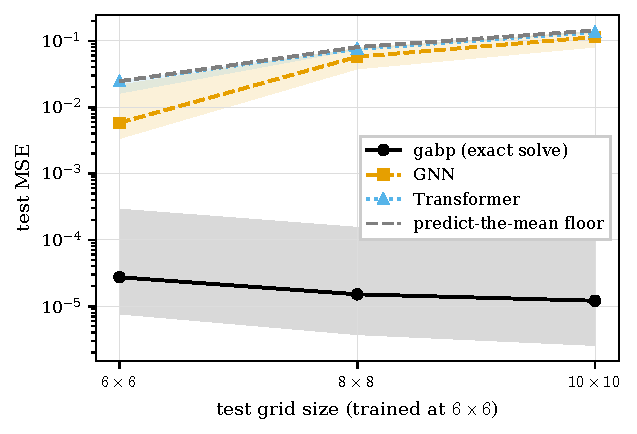
\includegraphics[width=\mazeextrapolationwidth]{figures/maze_extrapolation.pdf}
  \caption{Test error vs.\ grid size. Lines are medians over seeds 0--2, and
  bands span the corresponding minima and maxima. The exact-solve median
  remains below $10^{-4}$; the tested GNN and Transformer approach the
  predict-the-mean baseline. Data:
  \url{paper/attainability/figures/data/maze_extrapolation.csv}.}
  \label{fig:maze}
\end{figure}
\FloatBarrier

\paragraph{Within-architecture control: the effect is the solve's globality, not the
architecture.}
The much larger baselines show that the observed gap is not explained by raw
trainable-parameter count alone, but they differ in architecture and
optimization, so the gap could still be architectural. To isolate the
computation, the within-architecture intervention holds the \texttt{gabp}
model identical (same encoder, same
parameter count, same data and optimizer) and replaces its exact
\texttt{junction\_solve} with $K$ damped-Jacobi sweeps on the same learned
precision $A$. Starting from zero, each sweep expands point-source support by
at most one graph edge; after $K$ sweeps the sharp bound is $K-1$ edges. For
the convergent splitting used here, $K\to\infty$ recovers the exact solve; the
intervened variable is the iteration budget. The error decreases monotonically
with that budget
(Table~\ref{tab:maze-causal}, Figure~\ref{fig:maze-causal}): every displayed
finite-budget variant is worse than predict-the-mean (a truncated solve yields
a confidently wrong near-source field), and only the exact, global solve is
below that baseline. Its error is more than three orders of magnitude below
the deepest truncation. A matched-fit check on the held-out seeds (below)
shows why: the
preregistered $K=7$ arm cannot reach the exact arm's \emph{training} fit
(median relative train-loss gap $\sim2000\times$), so this
dose-response is best read as an attainability/optimization gap: the
finite truncations tested do not reproduce the globally coupled target.
It is not evidence that exactness biases training toward a
better solution among equally attainable ones.

\begin{table}[htbp]
  \centering
  \caption{Within-architecture Jacobi-budget control at $6\times6$; only the solve
  changes. Central processing unit (CPU), 64-bit floating-point (fp64), seed
  0. Displayed values are rounded conservatively
  against the exact-solve arm. Data:
  \url{paper/attainability/figures/data/maze_causal.csv}.}
  \label{tab:maze-causal}
  \begin{tabular}{lccccccc}
    \toprule
    Jacobi sweeps $K$ & 1 & 2 & 4 & 8 & 16 & 32 & exact \\
    \midrule
    test MSE & $2.9\mathrm{e}{-1}$ & $2.5\mathrm{e}{-1}$ & $2.1\mathrm{e}{-1}$ & $1.6\mathrm{e}{-1}$ & $1.0\mathrm{e}{-1}$ & $5.2\mathrm{e}{-2}$ & $\mathbf{1.2\mathrm{e}{-5}}$ \\
    \bottomrule
  \end{tabular}
\end{table}

\providecommand{\mazecausalwidth}{0.72\textwidth}
\begin{figure}[htbp]
  \centering
  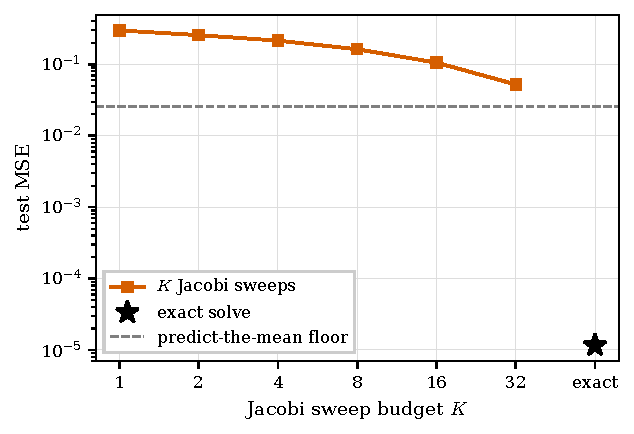
\includegraphics[width=\mazecausalwidth]{figures/maze_causal.pdf}
  \caption{Within-architecture Jacobi-budget control. Test error decreases with
  Jacobi depth $K$, but the finite variants do not attain the exact arm's
  training fit. Data:
  \url{paper/attainability/figures/data/maze_causal.csv}.}
  \label{fig:maze-causal}
\end{figure}

\paragraph{Preregistered matched-fit result on held-out seeds.}
The confirmatory test ran the routed-field task at sizes $6\times6$ to
$48\times48$ on $30$ reserved held-out seeds ($1000$--$1029$), comparing the
exact solve against a compute-matched truncated (Jacobi) baseline within the
same model class, under matched-fit decision rules frozen before the run
(thresholds predeclared in
\url{archive/docs/PREREGISTRATION_MATCHED_FIT_CONFIRMATORY.md}; the
confirmatory gates and per-cell adjudication are recorded in
\url{archive/docs/CONFIRMATORY_RESULTS.md}). The preselected $K=7$ arm is
\textbf{unmatchable for all $30$ seeds}: median exact training loss
$1.45\times10^{-5}$ against that arm's best of $2.96\times10^{-2}$,
a relative gap of about $2000\times$. Thus no matched-fit regime exists for
the confirmatory arm, supporting an attainability reading rather than a
preference among equally fit models. The
as-trained gap also shrinks with size ($8.17\times10^{-2}$ at size $6$ to
$1.30\times10^{-3}$ at size $48$), so there is no growing-extrapolation
signal beyond the attainability gap itself.
\providecommand{\tmlrevidencestart}{}
\providecommand{\tmlrevidenceend}{}
\tmlrevidencestart
Full verdict and per-seed records:
\url{archive/docs/CONFIRMATORY_RESULTS.md} (Maze section),
\url{archive/results/CONFIRMATORY/matched_fit_taskA/maze_matched_fit.json},
and \url{archive/results/CONFIRMATORY/matched_fit_taskA/maze_seeds/}.
\tmlrevidenceend
The $K=256$ floor arm's mean absolute extrapolation gaps are 3.8--4.6 orders
below the $K=7$ gaps, which is the comparison the frozen results prose used to mark
maze NC2 as passing. However, the same first-read JSON records
\texttt{floor\_sound=false}: at size 6, the mean floor-minus-exact loss gap is
$2.70\times10^{-5}$, or $44\%$ of the exact arm's mean evaluation loss,
against the implementation's separate $5\%$ in-distribution diagnostic.
Because the preregistration says ``function/extrapolation distance'' without
resolving these two checks, the manuscript treats the maze near-exact control
(NC2) as ambiguous, not as a clean pass.

\paragraph{Interpretation and scope.}
The task is solve-shaped by construction: the label is the output of a
structured global solve, and the \texttt{gabp} model contains that operator.
This accounts for the observed advantage over the tested GNN and Transformer
baselines. The preregistered matched-fit evidence does not establish
the stronger inductive-bias reading: that among models capable of comparably
fitting the training data, embedding the exact solve is what tips training
toward the generalizing one. The bounded-reach and message-passing
alternatives here are not comparably capable at these budgets; they do not
fit the target in the hard regime, which is an attainability/optimization
gap, not evidence of an implicit training preference.
Section~\ref{sec:program} states the benchmark-scale version and what would
falsify or refine this reading.

\section{Probe 2: stiff-regime training with exact implicit gradients}
\label{sec:deq}

The second axis is stability. A model's optimum can lie where the underlying
fixed point is stiff: long memory, strong coupling, slow mixing. Finite
unaccelerated gradient estimates can become inaccurate there. This section
shows that the exact selected-inverse backward keeps gradients correct in the
tested regime, so it can train where the tested finite Neumann adjoints do not.

\paragraph{The operator's role.}
A deep-equilibrium layer defines its output as a fixed point
$z^\star = f(z^\star, x)$. The implicit function theorem makes its backward
pass a single non-symmetric solve with the equilibrium Jacobian
$J=\partial f/\partial z$,
\begin{equation}
  (I-J)\T u = \partial\loss/\partial z^\star,
  \qquad \partial\loss/\partial\theta = u\T \,\partial f/\partial\theta .
  \label{eq:ift}
\end{equation}
When the coupling of $f$ is sparse on a low-treewidth graph, which is this
paper's regime, \eqref{eq:ift} is exactly the non-symmetric junction solve
sibling of selected inversion on $A = I-J$: one block $LDU$ factorization at
$\Theta(Wb^3)$ structural work,
with the transposed factor roles giving the adjoint without a second factorization
(Remark~\ref{rem:scaffold}). Common DEQ implementations obtain the adjoint
iteratively; the transparent baseline here uses
$u_{k+1} = J\T u_k + g$. After $K$ terms, the
Neumann tail is $(J\T)^K u^\star$; its asymptotic rate is governed by
$\rho(J)$, with constants and transients affected by non-normality. Thus the
unaccelerated iteration can become arbitrarily slow as $\rho(J)\to1$.

\paragraph{Result on four tested $\rho$ values: sparse direct remains accurate; finite
Neumann truncations degrade.}
On a non-symmetric coupling on a loopy $3\times3$ grid (genuine fill) scaled
to a target spectral radius, the experiment measures the parameter-gradient relative error
against a dense implicit-differentiation oracle (Table~\ref{tab:deq},
Figure~\ref{fig:deq}). The sparse-direct backward stays within
$1.1\times10^{-12}$ of the dense fp64 oracle on these four cells. Its error
rises as the system becomes nearly singular, as ordinary condition-sensitive
direct-solve analysis predicts. The iterative
backward degrades with the Neumann tail: at $\rho=0.99$ even $32$ terms leave
relative gradient error $77.1\%$, and at $\rho=0.999$ the error is $97.4\%$.
Separate unit tests validate the nonlinear implicit-function-theorem
backward against autograd through an unrolled solver
(\url{tests/test_deq_fixedpoint.py}).

\begin{table}[htbp]
  \centering
  \caption{Parameter-gradient relative error against a dense
  implicit-differentiation oracle as $\rho(J)\to1$. One deterministic instance
  per spectral radius, seed 0; central processing unit (CPU), 64-bit
  floating-point (fp64). Displayed values are rounded
  conservatively against sparse direct. Data:
  \url{paper/attainability/figures/data/deq_robustness.csv}.}
  \label{tab:deq}
  \begin{tabular}{rcccc}
    \toprule
    $\rho(J)$ & sparse direct & Neumann-8 & Neumann-16 & Neumann-32 \\
    \midrule
    $0.500$ & $\mathbf{1.83\mathrm{e}{-16}}$ & $1.17\mathrm{e}{-2}$ & $4.99\mathrm{e}{-5}$ & $7.55\mathrm{e}{-10}$ \\
    $0.900$ & $\mathbf{5.15\mathrm{e}{-16}}$ & $6.69\mathrm{e}{-1}$ & $3.05\mathrm{e}{-1}$ & $5.63\mathrm{e}{-2}$ \\
    $0.990$ & $\mathbf{1.65\mathrm{e}{-14}}$ & $9.74\mathrm{e}{-1}$ & $9.06\mathrm{e}{-1}$ & $7.71\mathrm{e}{-1}$ \\
    $0.999$ & $\mathbf{1.08\mathrm{e}{-12}}$ & $9.97\mathrm{e}{-1}$ & $9.90\mathrm{e}{-1}$ & $9.74\mathrm{e}{-1}$ \\
    \bottomrule
  \end{tabular}
\end{table}

\begin{figure}[t]
  \centering
  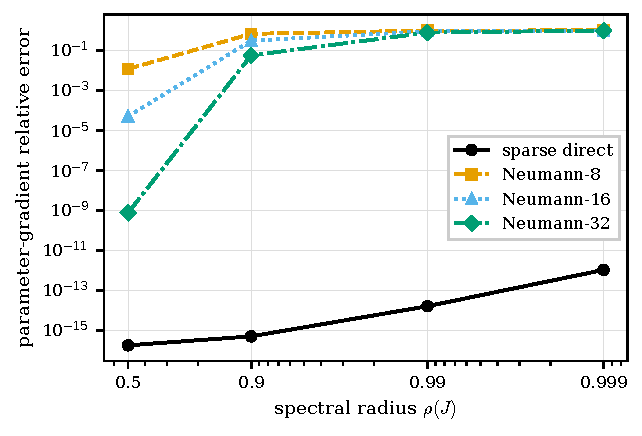
\includegraphics[width=0.72\textwidth]{figures/deq_robustness.pdf}
  \caption{Implicit-gradient error for sparse direct and finite Neumann
  adjoints. One deterministic instance is shown at each spectral radius;
  this is a finite diagnostic, not a
  condition-independent stability claim. Data:
  \url{paper/attainability/figures/data/deq_robustness.csv}.}
  \label{fig:deq}
\end{figure}

\paragraph{Confirmatory training-level test on held-out seeds.}
The gradient-error measurement above is exploratory, so a confirmatory,
training-level version of the claim was preregistered and run once on $30$
reserved held-out seeds ($1000$--$1029$) on their first aggregate read. Both
arms train a scalar gain through the same exact forward
solve ($n=16$, non-symmetric coupling), held bit-identical between arms; the
only intervention is the backward rule used during training, the exact
implicit adjoint versus a biased $K$-term Neumann adjoint. The
preregistered matched-fit adjudication
(\url{archive/bench/matched_fit_taskA.py}) distinguishes an equal-fit
preference from attainability by checking whether the Neumann arm can match the
exact arm's training loss (gated by a frozen floor and a $60\%$ matchability
bar) before crediting any test-loss gap to an inductive-bias mechanism. In
the stiff cells ($\rho\in\{0.98,0.99\}$ and $K\in\{1,2,4\}$) the
Neumann arm is matchable in only $0$--$23.3\%$ of seeds
(relative train gap $+1.45$ to $+13.2$), so the inductive-bias
(\textsc{survive}) branch has nothing to compare there; the result resolves to
the conservative attainability/optimization reading. That branch is also
unreachable at the one high-$\rho$ arm that does clear the matchability bar,
because that arm calibrates the floor it would have to exceed; this is a
defect of the frozen rule rather than a finding, and
Appendix~\ref{app:integrity} states it. The one designed silent
control ($\rho=0.5$) did not cleanly pass: its relative-gap clause failed
(driven by a denominator-scale instability in the relative ratio, with both arms
converging to losses of order $10^{-8}$--$10^{-9}$), though its
independent function-distance clause passed by more than four orders of
magnitude. Per the frozen rule (a positive reading is void unless its
negative controls hold), this is reported as a hedged, not pristine,
conservative verdict, not relaxed after the fact. Full adjudication, per-cell
table, and per-seed records:
\url{archive/docs/CONFIRMATORY_RESULTS.md},
\url{archive/docs/PREREGISTRATION_MATCHED_FIT_CONFIRMATORY.md}, and
\url{archive/results/CONFIRMATORY/matched_fit_taskA/deq_matched_fit.json}.

A later branch reused the same HOLDOUT seeds for a different bootstrap
analysis after this first read. That second use is not an independent
confirmation, and none of its verdicts or effect-size claims is used here.
Appendix~\ref{app:integrity} records the chronology and a nested run-tag
metadata defect.

\paragraph{Interpretation and scope.}
The error sweep is a mechanism result at controlled scale ($n=9$): it shows
the exact sparse-direct backward is accurate on the tested cells where the
finite Neumann truncation is not, and that the training arms differ in
attainability under the first-read protocol. The adjudication does not support
the stronger claim that this difference reflects an inductive bias among
equally attainable optima, because the hard cells do not supply an equal-fit
comparison. On this evidence, the observed difference reflects the iterative
arm's inability to fit the stiff cells, an attainability/optimization effect
rather than a preference effect. Neumann iteration is the transparent
baseline; accelerated solvers (Anderson \citep{anderson1965iterative} and
Broyden \citep{broyden1965class}) can reduce the iteration count and are
necessary competitors at scale; they were not evaluated here. The structured
direct solve avoids a convergence tolerance but retains ordinary
conditioning-dependent rounding error. The affine diagnostic uses a
convergent construction with $\rho(J)<1$; the advantage is for
graph-structured, low-treewidth Jacobians. For a dense $J$, the $LDU$
factorization is $\bigO(n^3)$ and an
iterative method may be preferable. A benchmark-scale learned-capability gain
has not been demonstrated and would need its own matched-fit or attainability
control for a valid attribution.
